\documentclass[tikz,border=8pt]{standalone}
% Shared look for every TikZ diagram. Load with \input{../../tools/tikz-style.tex}
\usepackage[T1]{fontenc}
\usepackage{lmodern}
\renewcommand{\sfdefault}{lmr}  % diagrams use the same serif as the text
\usetikzlibrary{arrows.meta, positioning, shapes.geometric, calc, fit, backgrounds}
\definecolor{cblue}{HTML}{4C78A8}
\definecolor{corange}{HTML}{F58518}
\definecolor{cgreen}{HTML}{54A24B}
\definecolor{cred}{HTML}{E45756}
\definecolor{cpurple}{HTML}{B279A2}
\definecolor{cgrey}{HTML}{6B6B6B}
\tikzset{
  every picture/.style={font=\sffamily, line width=1.2pt},
  box/.style={draw=#1, fill=#1!12, rounded corners=4pt, align=center, inner sep=7pt, minimum height=1.1cm},
  box/.default=cgrey,
  arrow/.style={-{Stealth[length=3mm]}, draw=cgrey, line width=1.4pt},
  title/.style={font=\sffamily\bfseries\Large},
  note/.style={font=\sffamily\small, text=cgrey, align=center},
}
\AtBeginDocument{\hyphenpenalty=10000 \exhyphenpenalty=10000}

\usetikzlibrary{matrix}
\begin{document}
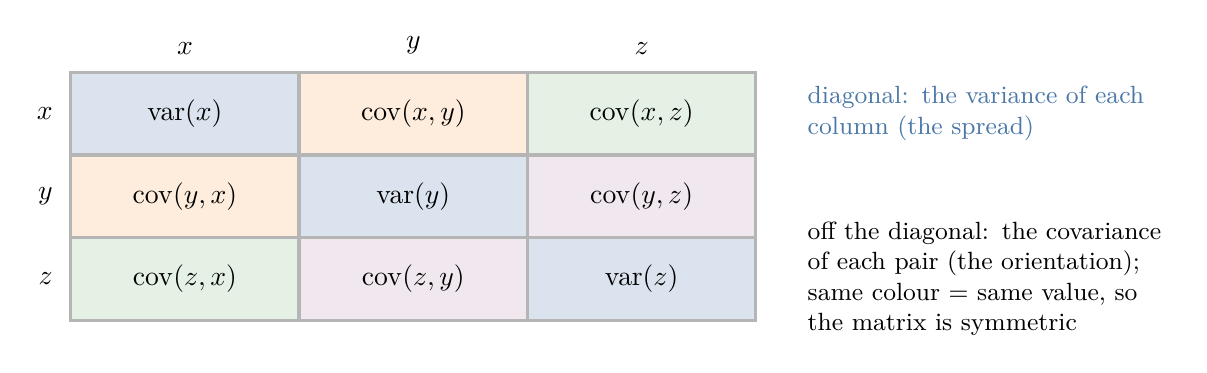
\begin{tikzpicture}
  \matrix (m) [matrix of math nodes, column sep=-\pgflinewidth, row sep=-\pgflinewidth,
     nodes={minimum width=2.9cm, minimum height=1.05cm, anchor=center, draw=cgrey!50, font=\normalsize}]
  { |[fill=cblue!20]| \mathrm{var}(x) & |[fill=corange!15]| \mathrm{cov}(x,y) & |[fill=cgreen!15]| \mathrm{cov}(x,z) \\
    |[fill=corange!15]| \mathrm{cov}(y,x) & |[fill=cblue!20]| \mathrm{var}(y) & |[fill=cpurple!18]| \mathrm{cov}(y,z) \\
    |[fill=cgreen!15]| \mathrm{cov}(z,x) & |[fill=cpurple!18]| \mathrm{cov}(z,y) & |[fill=cblue!20]| \mathrm{var}(z) \\ };
  \foreach \c/\n in {1/x,2/y,3/z} {
    \node[above=2pt of m-1-\c, font=\bfseries] {$\n$};
    \node[left=2pt of m-\c-1, font=\bfseries] {$\n$};
  }
  \node[note, right=0.5cm of m-1-3, text width=4.6cm, align=left, text=cblue] {diagonal: the variance of each column (the spread)};
  \node[note, right=0.5cm of m-3-3, text width=4.6cm, align=left, text=black] {off the diagonal: the covariance of each pair (the orientation); same colour = same value, so the matrix is symmetric};
\end{tikzpicture}
\end{document}
